% Options for packages loaded elsewhere
% Options for packages loaded elsewhere
\PassOptionsToPackage{unicode}{hyperref}
\PassOptionsToPackage{hyphens}{url}
\PassOptionsToPackage{dvipsnames,svgnames,x11names}{xcolor}
%
\documentclass[
  spanish,
  11pt,
  letterpaper,
]{book}
\usepackage{xcolor}
\usepackage[margin=2.5cm]{geometry}
\usepackage{amsmath,amssymb}
\setcounter{secnumdepth}{5}
\usepackage{iftex}
\ifPDFTeX
  \usepackage[T1]{fontenc}
  \usepackage[utf8]{inputenc}
  \usepackage{textcomp} % provide euro and other symbols
\else % if luatex or xetex
  \usepackage{unicode-math} % this also loads fontspec
  \defaultfontfeatures{Scale=MatchLowercase}
  \defaultfontfeatures[\rmfamily]{Ligatures=TeX,Scale=1}
\fi
\usepackage{lmodern}
\ifPDFTeX\else
  % xetex/luatex font selection
\fi
% Use upquote if available, for straight quotes in verbatim environments
\IfFileExists{upquote.sty}{\usepackage{upquote}}{}
\IfFileExists{microtype.sty}{% use microtype if available
  \usepackage[]{microtype}
  \UseMicrotypeSet[protrusion]{basicmath} % disable protrusion for tt fonts
}{}
\makeatletter
\@ifundefined{KOMAClassName}{% if non-KOMA class
  \IfFileExists{parskip.sty}{%
    \usepackage{parskip}
  }{% else
    \setlength{\parindent}{0pt}
    \setlength{\parskip}{6pt plus 2pt minus 1pt}}
}{% if KOMA class
  \KOMAoptions{parskip=half}}
\makeatother
% Make \paragraph and \subparagraph free-standing
\makeatletter
\ifx\paragraph\undefined\else
  \let\oldparagraph\paragraph
  \renewcommand{\paragraph}{
    \@ifstar
      \xxxParagraphStar
      \xxxParagraphNoStar
  }
  \newcommand{\xxxParagraphStar}[1]{\oldparagraph*{#1}\mbox{}}
  \newcommand{\xxxParagraphNoStar}[1]{\oldparagraph{#1}\mbox{}}
\fi
\ifx\subparagraph\undefined\else
  \let\oldsubparagraph\subparagraph
  \renewcommand{\subparagraph}{
    \@ifstar
      \xxxSubParagraphStar
      \xxxSubParagraphNoStar
  }
  \newcommand{\xxxSubParagraphStar}[1]{\oldsubparagraph*{#1}\mbox{}}
  \newcommand{\xxxSubParagraphNoStar}[1]{\oldsubparagraph{#1}\mbox{}}
\fi
\makeatother


\usepackage{longtable,booktabs,array}
\newcounter{none} % for unnumbered tables
\usepackage{calc} % for calculating minipage widths
% Correct order of tables after \paragraph or \subparagraph
\usepackage{etoolbox}
\makeatletter
\patchcmd\longtable{\par}{\if@noskipsec\mbox{}\fi\par}{}{}
\makeatother
% Allow footnotes in longtable head/foot
\IfFileExists{footnotehyper.sty}{\usepackage{footnotehyper}}{\usepackage{footnote}}
\makesavenoteenv{longtable}
\usepackage{graphicx}
\makeatletter
\newsavebox\pandoc@box
\newcommand*\pandocbounded[1]{% scales image to fit in text height/width
  \sbox\pandoc@box{#1}%
  \Gscale@div\@tempa{\textheight}{\dimexpr\ht\pandoc@box+\dp\pandoc@box\relax}%
  \Gscale@div\@tempb{\linewidth}{\wd\pandoc@box}%
  \ifdim\@tempb\p@<\@tempa\p@\let\@tempa\@tempb\fi% select the smaller of both
  \ifdim\@tempa\p@<\p@\scalebox{\@tempa}{\usebox\pandoc@box}%
  \else\usebox{\pandoc@box}%
  \fi%
}
% Set default figure placement to htbp
\def\fps@figure{htbp}
\makeatother



\ifLuaTeX
\usepackage[bidi=basic,shorthands=off]{babel}
\else
\usepackage[bidi=default,shorthands=off]{babel}
\fi
\ifLuaTeX
  \usepackage{selnolig} % disable illegal ligatures
\fi


\setlength{\emergencystretch}{3em} % prevent overfull lines

\providecommand{\tightlist}{%
  \setlength{\itemsep}{0pt}\setlength{\parskip}{0pt}}



 


\usepackage{xcolor}
\usepackage{titlesec}
\definecolor{AzulLibro}{HTML}{0B4F6C}
\definecolor{TurquesaLibro}{HTML}{0EA5A8}
\definecolor{GrisTexto}{HTML}{374151}
\renewcommand{\contentsname}{Índice general}
\renewcommand{\chaptername}{Capítulo}
\titleformat{\chapter}[display]
  {\normalfont\huge\bfseries\color{AzulLibro}}
  {\chaptername\ \thechapter}{16pt}{\Huge}
\titleformat{\section}
  {\normalfont\Large\bfseries\color{AzulLibro}}
  {\thesection}{1em}{}
\titleformat{\subsection}
  {\normalfont\large\bfseries\color{TurquesaLibro}}
  {\thesubsection}{1em}{}
\makeatletter
\@ifpackageloaded{tcolorbox}{}{\usepackage[skins,breakable]{tcolorbox}}
\@ifpackageloaded{fontawesome5}{}{\usepackage{fontawesome5}}
\definecolor{quarto-callout-color}{HTML}{909090}
\definecolor{quarto-callout-note-color}{HTML}{0758E5}
\definecolor{quarto-callout-important-color}{HTML}{CC1914}
\definecolor{quarto-callout-warning-color}{HTML}{EB9113}
\definecolor{quarto-callout-tip-color}{HTML}{00A047}
\definecolor{quarto-callout-caution-color}{HTML}{FC5300}
\definecolor{quarto-callout-color-frame}{HTML}{acacac}
\definecolor{quarto-callout-note-color-frame}{HTML}{4582ec}
\definecolor{quarto-callout-important-color-frame}{HTML}{d9534f}
\definecolor{quarto-callout-warning-color-frame}{HTML}{f0ad4e}
\definecolor{quarto-callout-tip-color-frame}{HTML}{02b875}
\definecolor{quarto-callout-caution-color-frame}{HTML}{fd7e14}
\makeatother
\makeatletter
\@ifpackageloaded{bookmark}{}{\usepackage{bookmark}}
\makeatother
\makeatletter
\@ifpackageloaded{caption}{}{\usepackage{caption}}
\AtBeginDocument{%
\ifdefined\contentsname
  \renewcommand*\contentsname{Tabla de contenidos}
\else
  \newcommand\contentsname{Tabla de contenidos}
\fi
\ifdefined\listfigurename
  \renewcommand*\listfigurename{Listado de Figuras}
\else
  \newcommand\listfigurename{Listado de Figuras}
\fi
\ifdefined\listtablename
  \renewcommand*\listtablename{Listado de Tablas}
\else
  \newcommand\listtablename{Listado de Tablas}
\fi
\ifdefined\figurename
  \renewcommand*\figurename{Figura}
\else
  \newcommand\figurename{Figura}
\fi
\ifdefined\tablename
  \renewcommand*\tablename{Tabla}
\else
  \newcommand\tablename{Tabla}
\fi
}
\@ifpackageloaded{float}{}{\usepackage{float}}
\floatstyle{ruled}
\@ifundefined{c@chapter}{\newfloat{codelisting}{h}{lop}}{\newfloat{codelisting}{h}{lop}[chapter]}
\floatname{codelisting}{Listado}
\newcommand*\listoflistings{\listof{codelisting}{Listado de Listados}}
\makeatother
\makeatletter
\makeatother
\makeatletter
\@ifpackageloaded{caption}{}{\usepackage{caption}}
\@ifpackageloaded{subcaption}{}{\usepackage{subcaption}}
\makeatother
\makeatletter
\@ifpackageloaded{tcolorbox}{}{\usepackage[skins,breakable]{tcolorbox}}
\makeatother
\makeatletter
\@ifundefined{shadecolor}{\definecolor{shadecolor}{HTML}{0B4F6C}}{}
\makeatother
\makeatletter
\@ifundefined{codebgcolor}{\definecolor{codebgcolor}{HTML}{F3F7FA}}{}
\makeatother
\makeatletter
\ifdefined\Shaded\renewenvironment{Shaded}{\begin{tcolorbox}[borderline west={3pt}{0pt}{shadecolor}, boxrule=0pt, breakable, colback={codebgcolor}, enhanced, frame hidden, sharp corners]}{\end{tcolorbox}}\fi
\makeatother
\usepackage{bookmark}
\IfFileExists{xurl.sty}{\usepackage{xurl}}{} % add URL line breaks if available
\urlstyle{same}
\hypersetup{
  pdftitle={Aprendizaje y Clasificación Automática con R},
  pdfauthor={MI Jesús Gilberto Rodríguez Escobedo},
  pdflang={es},
  colorlinks=true,
  linkcolor={Maroon},
  filecolor={Maroon},
  citecolor={Blue},
  urlcolor={Blue},
  pdfcreator={LaTeX via pandoc}}


\title{Aprendizaje y Clasificación Automática con R}
\usepackage{etoolbox}
\makeatletter
\providecommand{\subtitle}[1]{% add subtitle to \maketitle
  \apptocmd{\@title}{\par {\large #1 \par}}{}{}
}
\makeatother
\subtitle{Un enfoque práctico con datos abiertos reales}
\author{MI Jesús Gilberto Rodríguez Escobedo}
\date{2026-07-10}
\begin{document}
\frontmatter
\maketitle

\renewcommand*\contentsname{Índice general}
{
\setcounter{tocdepth}{2}
\tableofcontents
}

\mainmatter
\bookmarksetup{startatroot}

\chapter*{Presentación}\label{presentaciuxf3n}
\addcontentsline{toc}{chapter}{Presentación}

\markboth{Presentación}{Presentación}

\section*{Aprendizaje y Clasificación Automática con
R}\label{aprendizaje-y-clasificaciuxf3n-automuxe1tica-con-r}
\addcontentsline{toc}{section}{Aprendizaje y Clasificación Automática
con R}

\markright{Aprendizaje y Clasificación Automática con R}

\subsection*{Un enfoque práctico con datos abiertos
reales}\label{un-enfoque-pruxe1ctico-con-datos-abiertos-reales}
\addcontentsline{toc}{subsection}{Un enfoque práctico con datos abiertos
reales}

\textbf{Autor:} MI Jesús Gilberto Rodríguez Escobedo\\
\textbf{Versión:} 0.5\\
\textbf{Modalidad:} Libro abierto, práctico e interactivo

\texttt{R} · \texttt{Quarto} · \texttt{Machine\ Learning} ·
\texttt{Datos\ abiertos} · \texttt{GitHub\ Pages}

Este libro introduce el aprendizaje automático (\emph{Machine Learning})
mediante ejemplos claros, didácticos y prácticos desarrollados
principalmente en R.

La intención no es escribir un tratado matemático extenso, sino
construir una guía aplicada para aprender haciendo con datos abiertos
reales. En esta versión trabajamos con datos de accidentes de tránsito
de México y los usamos como hilo conductor para explicar preparación de
datos, análisis exploratorio y modelos de clasificación.

\begin{tcolorbox}[enhanced jigsaw, arc=.35mm, bottomrule=.15mm, bottomtitle=1mm, breakable, colback=white, colbacktitle=quarto-callout-tip-color!10!white, colframe=quarto-callout-tip-color-frame, coltitle=black, left=2mm, leftrule=.75mm, opacityback=0, opacitybacktitle=0.6, rightrule=.15mm, title=\textcolor{quarto-callout-tip-color}{\faLightbulb}\hspace{0.5em}{Enfoque del libro}, titlerule=0mm, toprule=.15mm, toptitle=1mm]

El libro combina fundamento conceptual, código reproducible en R,
interpretación didáctica de resultados y visualizaciones profesionales.

\end{tcolorbox}

\section*{Objetivo general}\label{objetivo-general}
\addcontentsline{toc}{section}{Objetivo general}

\markright{Objetivo general}

Desarrollar competencias básicas e intermedias en aprendizaje automático
mediante el análisis, modelado e interpretación de datos reales.

\section*{Público al que va
dirigido}\label{puxfablico-al-que-va-dirigido}
\addcontentsline{toc}{section}{Público al que va dirigido}

\markright{Público al que va dirigido}

Este libro está dirigido a estudiantes de ingeniería, ciencias, ciencia
de datos, estadística aplicada y áreas afines que desean iniciar en
aprendizaje automático con un enfoque práctico.

\section*{Software utilizado}\label{software-utilizado}
\addcontentsline{toc}{section}{Software utilizado}

\markright{Software utilizado}

Los ejemplos se desarrollan principalmente en R, usando RStudio y
Quarto. También se mencionan herramientas útiles para publicar y
compartir resultados:

\begin{itemize}
\tightlist
\item
  RStudio
\item
  Consola de R
\item
  Google Colab
\item
  GitHub
\item
  GitHub Pages
\item
  Quarto Pub
\end{itemize}

\section*{Estructura actual del
libro}\label{estructura-actual-del-libro}
\addcontentsline{toc}{section}{Estructura actual del libro}

\markright{Estructura actual del libro}

\begin{enumerate}
\def\labelenumi{\arabic{enumi}.}
\tightlist
\item
  Introducción al aprendizaje automático.
\item
  Preparación de datos reales.
\item
  Análisis exploratorio de datos.
\item
  Regresión logística.
\item
  k vecinos más cercanos.
\item
  Árboles de decisión.
\item
  Random Forest.
\end{enumerate}

\section*{Nota para el lector}\label{nota-para-el-lector}
\addcontentsline{toc}{section}{Nota para el lector}

\markright{Nota para el lector}

Los capítulos están diseñados para leerse y ejecutarse paso a paso. Cada
bloque de código busca responder una pregunta concreta y cada resultado
se acompaña de una interpretación didáctica.

\bookmarksetup{startatroot}

\chapter*{Licencia, autoría y forma de
citar}\label{licencia-autoruxeda-y-forma-de-citar}
\addcontentsline{toc}{chapter}{Licencia, autoría y forma de citar}

\markboth{Licencia, autoría y forma de citar}{Licencia, autoría y forma
de citar}

\section*{Autor}\label{autor}
\addcontentsline{toc}{section}{Autor}

\markright{Autor}

\textbf{MI Jesús Gilberto Rodríguez Escobedo}

\section*{Licencia}\label{licencia}
\addcontentsline{toc}{section}{Licencia}

\markright{Licencia}

Este libro se distribuye bajo la licencia \textbf{Creative Commons
Atribución-NoComercial-CompartirIgual 4.0 Internacional (CC BY-NC-SA
4.0)}.

Esto significa que el material puede compartirse y adaptarse con fines
educativos y no comerciales, siempre que se otorgue el crédito
correspondiente al autor y las obras derivadas se compartan bajo una
licencia compatible.

\section*{Cita sugerida}\label{cita-sugerida}
\addcontentsline{toc}{section}{Cita sugerida}

\markright{Cita sugerida}

Rodríguez Escobedo, J. G. (2026). \emph{Aprendizaje y Clasificación
Automática con R: Un enfoque práctico con datos abiertos reales}. Libro
web publicado con Quarto y GitHub Pages.

\section*{Uso educativo}\label{uso-educativo}
\addcontentsline{toc}{section}{Uso educativo}

\markright{Uso educativo}

El propósito de este libro es apoyar la enseñanza y el aprendizaje de
técnicas de aprendizaje automático con R, usando datos reales y un
enfoque didáctico, reproducible y aplicado.

\bookmarksetup{startatroot}

\chapter{¿Qué es el aprendizaje
automático?}\label{quuxe9-es-el-aprendizaje-automuxe1tico}

\section{Objetivos del capítulo}\label{objetivos-del-capuxedtulo}

Al finalizar este capítulo, el lector será capaz de explicar qué es el
aprendizaje automático, diferenciarlo de la programación tradicional e
identificar problemas de clasificación, regresión y agrupamiento.

\section{Introducción}\label{introducciuxf3n}

El aprendizaje automático, también conocido como \emph{Machine
Learning}, es una rama de la inteligencia artificial que permite
construir modelos capaces de aprender patrones a partir de datos.

En la programación tradicional, una persona define reglas. En
aprendizaje automático, proporcionamos ejemplos para que un algoritmo
aprenda una relación entre variables de entrada y una salida esperada.

\section{Programación tradicional contra aprendizaje
automático}\label{programaciuxf3n-tradicional-contra-aprendizaje-automuxe1tico}

\begin{verbatim}
[1] "Contaminación alta"
\end{verbatim}

\textbf{Interpretación.} Este ejemplo muestra programación tradicional:
la decisión depende de una regla escrita manualmente.

\begin{verbatim}
   dia pm10 temperatura humedad clase
1    1   42          25      40  Baja
2    2   88          28      35  Alta
3    3   55          22      60  Baja
4    4  120          30      30  Alta
5    5   63          24      55  Baja
6    6   95          29      33  Alta
7    7   38          21      65  Baja
8    8  110          31      29  Alta
9    9   72          27      42  Baja
10  10  130          32      28  Alta
11  11   47          23      62  Baja
12  12   99          30      34  Alta
\end{verbatim}

\section{Variables predictoras y variable
respuesta}\label{variables-predictoras-y-variable-respuesta}

La \textbf{variable respuesta} es la variable que queremos predecir. Las
\textbf{variables predictoras} son las variables que usamos como entrada
para el modelo.

\section{Tipos principales de aprendizaje
automático}\label{tipos-principales-de-aprendizaje-automuxe1tico}

\begin{enumerate}
\def\labelenumi{\arabic{enumi}.}
\tightlist
\item
  Aprendizaje supervisado.
\item
  Aprendizaje no supervisado.
\item
  Aprendizaje por refuerzo.
\end{enumerate}

\section{Notación básica}\label{notaciuxf3n-buxe1sica}

Supongamos que tenemos \(n\) observaciones y \(p\) variables
predictoras. Podemos representar los datos mediante una matriz \(X\) y
una variable respuesta \(Y\).

\[
\hat{y}=f(x_1,x_2,\ldots,x_p)
\]

\section{Primer ejemplo visual en R}\label{primer-ejemplo-visual-en-r}

\pandocbounded{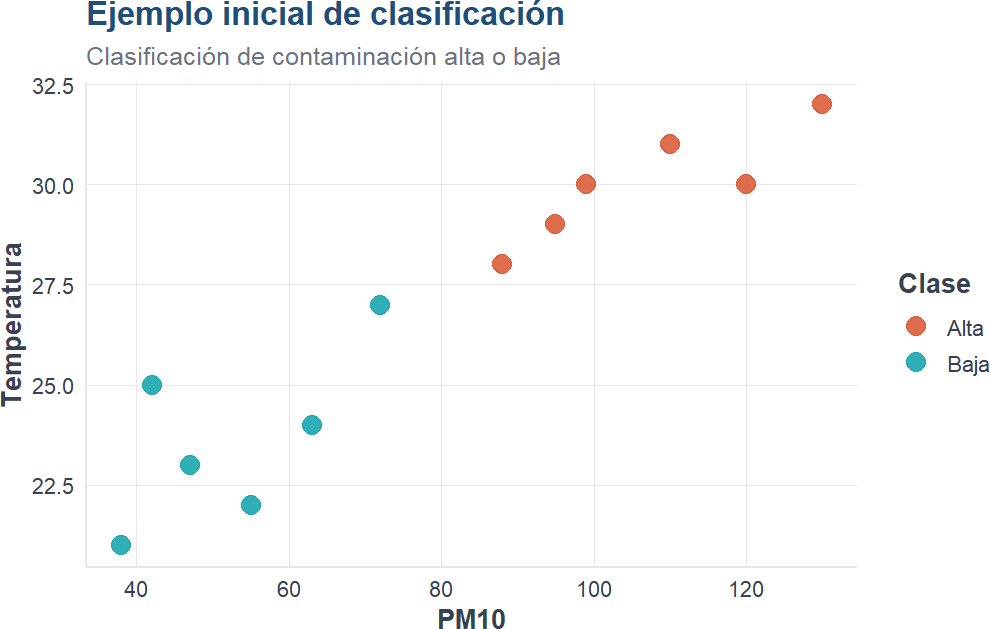
\includegraphics[keepaspectratio]{01-introduccion_files/figure-pdf/unnamed-chunk-3-1.png}}

\section{División entre entrenamiento y
prueba}\label{divisiuxf3n-entre-entrenamiento-y-prueba}

\begin{verbatim}
   dia pm10 temperatura humedad clase
3    3   55          22      60  Baja
12  12   99          30      34  Alta
10  10  130          32      28  Alta
2    2   88          28      35  Alta
6    6   95          29      33  Alta
11  11   47          23      62  Baja
5    5   63          24      55  Baja
4    4  120          30      30  Alta
\end{verbatim}

\begin{verbatim}
  dia pm10 temperatura humedad clase
1   1   42          25      40  Baja
7   7   38          21      65  Baja
8   8  110          31      29  Alta
9   9   72          27      42  Baja
\end{verbatim}

\section{Primer clasificador basado en una
regla}\label{primer-clasificador-basado-en-una-regla}

\begin{verbatim}
      Predicho
Real   Alta Baja
  Alta    6    0
  Baja    0    6
\end{verbatim}

\begin{verbatim}
[1] 1
\end{verbatim}

\section{Conclusión}\label{conclusiuxf3n}

El aprendizaje automático permite construir modelos que aprenden
patrones a partir de datos. En este capítulo vimos la diferencia entre
reglas manuales y aprendizaje a partir de ejemplos.

\bookmarksetup{startatroot}

\chapter{Preparación de datos
reales}\label{preparaciuxf3n-de-datos-reales}

\section{Objetivos del capítulo}\label{objetivos-del-capuxedtulo-1}

Al finalizar este capítulo, el lector será capaz de leer una base real,
seleccionar variables, construir una variable respuesta y guardar una
base preparada para modelado.

\section{Introducción}\label{introducciuxf3n-1}

En la práctica profesional, los datos reales casi nunca vienen
preparados. Antes de aplicar un algoritmo necesitamos revisar, limpiar,
transformar y documentar los datos.

\section{Cargar paquetes}\label{cargar-paquetes}

\section{Leer el archivo CSV}\label{leer-el-archivo-csv}

\begin{verbatim}
[1] TRUE
\end{verbatim}

\begin{verbatim}
[1] "Archivo leído correctamente."
\end{verbatim}

\section{Primer vistazo a los datos}\label{primer-vistazo-a-los-datos}

\begin{verbatim}
# A tibble: 6 x 45
  COBERTURA ID_ENTIDAD ID_MUNICIPIO  ANIO MES   ID_HORA ID_MINUTO ID_DIA
  <chr>     <chr>      <chr>        <dbl> <chr> <chr>   <chr>     <chr> 
1 Municipal 01         001           2024 01    02      25        01    
2 Municipal 01         001           2024 01    03      40        01    
3 Municipal 01         001           2024 01    04      37        01    
4 Municipal 01         001           2024 01    05      00        01    
5 Municipal 01         001           2024 01    06      45        01    
6 Municipal 01         001           2024 01    07      30        01    
# i 37 more variables: DIASEMANA <chr>, URBANA <chr>, SUBURBANA <chr>,
#   TIPACCID <chr>, AUTOMOVIL <dbl>, CAMPASAJ <dbl>, MICROBUS <dbl>,
#   PASCAMION <dbl>, OMNIBUS <dbl>, TRANVIA <dbl>, CAMIONETA <dbl>,
#   CAMION <dbl>, TRACTOR <dbl>, FERROCARRI <dbl>, MOTOCICLET <dbl>,
#   BICICLETA <dbl>, OTROVEHIC <dbl>, CAUSAACCI <chr>, CAPAROD <chr>,
#   SEXO <chr>, ALIENTO <chr>, CINTURON <chr>, ID_EDAD <dbl>, CONDMUERTO <dbl>,
#   CONDHERIDO <dbl>, PASAMUERTO <dbl>, PASAHERIDO <dbl>, PEATMUERTO <dbl>, ...
\end{verbatim}

\section{Variables de interés}\label{variables-de-interuxe9s}

\begin{verbatim}
# A tibble: 6 x 10
   ANIO MES   ID_ENTIDAD ID_MUNICIPIO ID_HORA ID_DIA DIASEMANA TIPACCID         
  <dbl> <chr> <chr>      <chr>        <chr>   <chr>  <chr>     <chr>            
1  2024 01    01         001          02      01     lunes     Colisión con veh~
2  2024 01    01         001          03      01     lunes     Colisión con obj~
3  2024 01    01         001          04      01     lunes     Colisión con pea~
4  2024 01    01         001          05      01     lunes     Colisión con obj~
5  2024 01    01         001          06      01     lunes     Colisión con obj~
6  2024 01    01         001          07      01     lunes     Colisión con veh~
# i 2 more variables: CAUSAACCI <chr>, CLASACC <chr>
\end{verbatim}

\section{Crear variable respuesta}\label{crear-variable-respuesta}

\begin{verbatim}

Con víctimas   Solo daños 
       68108       322519 
\end{verbatim}

\section{Preparar variables finales}\label{preparar-variables-finales}

\begin{verbatim}
   filas columnas
1 390627        6
\end{verbatim}

\section{Guardar base preparada}\label{guardar-base-preparada}

\section{Resumen del capítulo}\label{resumen-del-capuxedtulo}

En este capítulo leímos una base real, seleccionamos variables,
construimos una variable respuesta y guardamos una base preparada para
aprendizaje automático.

\bookmarksetup{startatroot}

\chapter{Análisis exploratorio de
datos}\label{anuxe1lisis-exploratorio-de-datos}

\section{Objetivos del capítulo}\label{objetivos-del-capuxedtulo-2}

Al finalizar este capítulo, el lector será capaz de cargar una base
preparada, revisar su estructura, calcular frecuencias, construir
gráficas e interpretar patrones iniciales.

\section{Cargar paquetes y base}\label{cargar-paquetes-y-base}

\begin{verbatim}
[1] "Base preparada cargada correctamente."
\end{verbatim}

\section{Preparar variables}\label{preparar-variables}

\section{Distribución de la variable
respuesta}\label{distribuciuxf3n-de-la-variable-respuesta}

\begin{verbatim}

Con víctimas   Solo daños 
       17.44        82.56 
\end{verbatim}

\pandocbounded{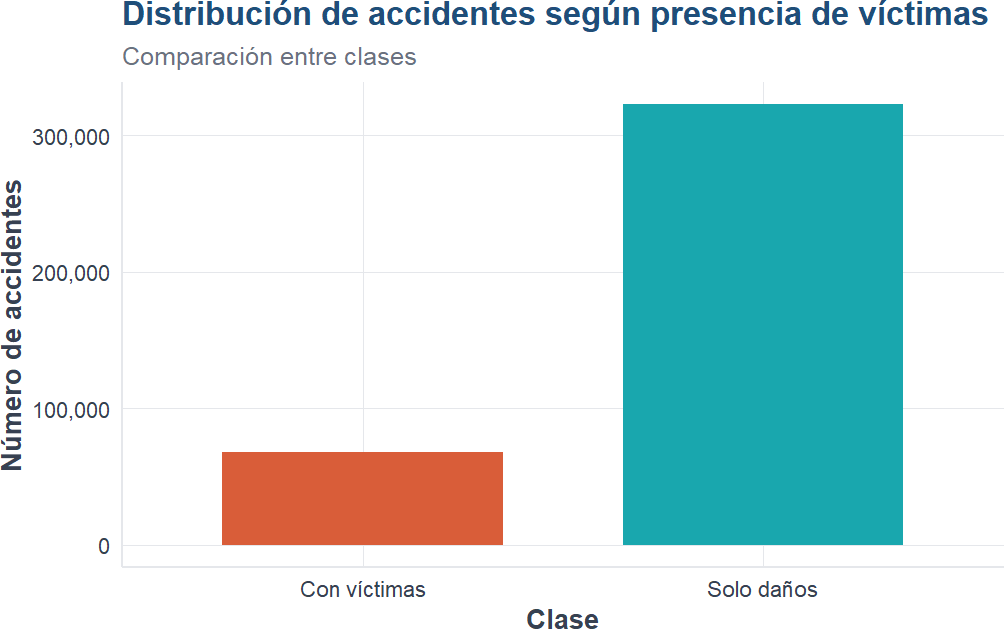
\includegraphics[keepaspectratio]{03-analisis-exploratorio_files/figure-pdf/unnamed-chunk-4-1.png}}

\section{Accidentes por mes}\label{accidentes-por-mes}

\begin{verbatim}
# A tibble: 12 x 2
   MES_FACTOR     n
   <fct>      <int>
 1 01         31600
 2 02         32208
 3 03         33237
 4 04         32666
 5 05         34665
 6 06         31737
 7 07         30062
 8 08         31800
 9 09         31351
10 10         33771
11 11         34047
12 12         33483
\end{verbatim}

\pandocbounded{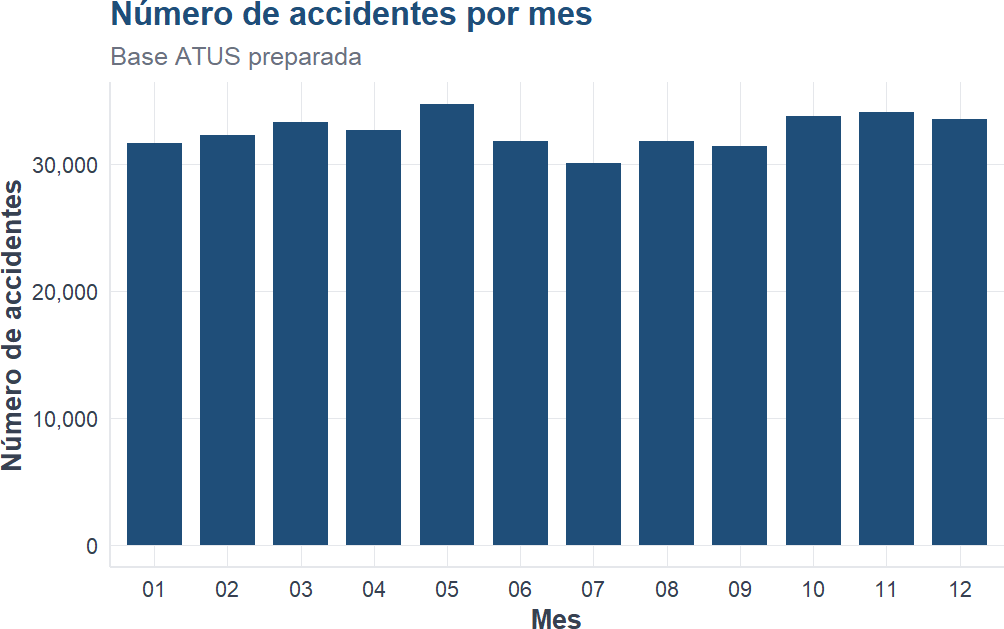
\includegraphics[keepaspectratio]{03-analisis-exploratorio_files/figure-pdf/unnamed-chunk-6-1.png}}

\section{Accidentes por hora del
día}\label{accidentes-por-hora-del-duxeda}

\pandocbounded{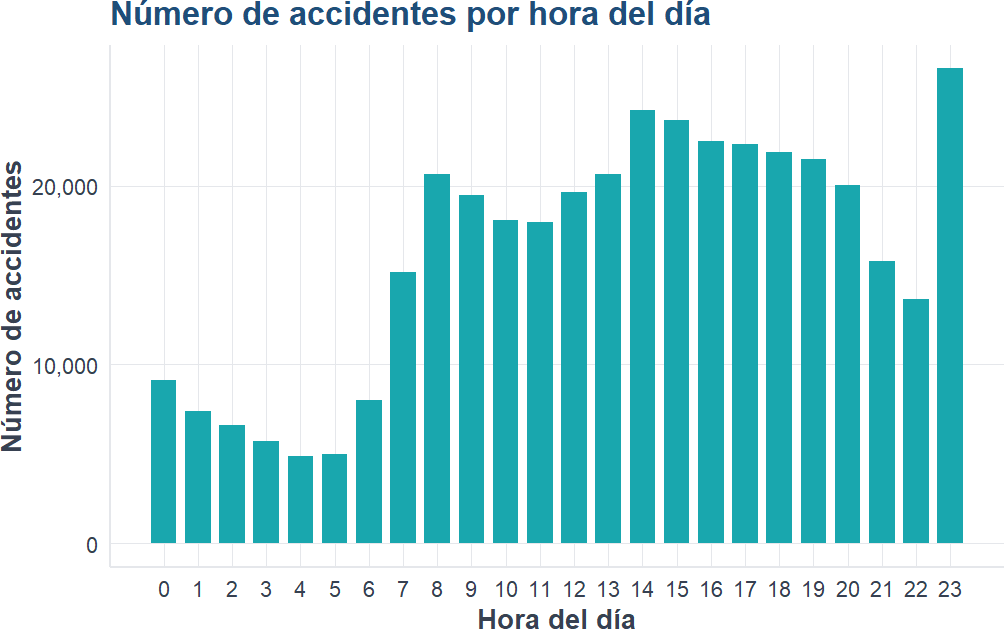
\includegraphics[keepaspectratio]{03-analisis-exploratorio_files/figure-pdf/unnamed-chunk-7-1.png}}

\section{Tipos de accidente más
frecuentes}\label{tipos-de-accidente-muxe1s-frecuentes}

\pandocbounded{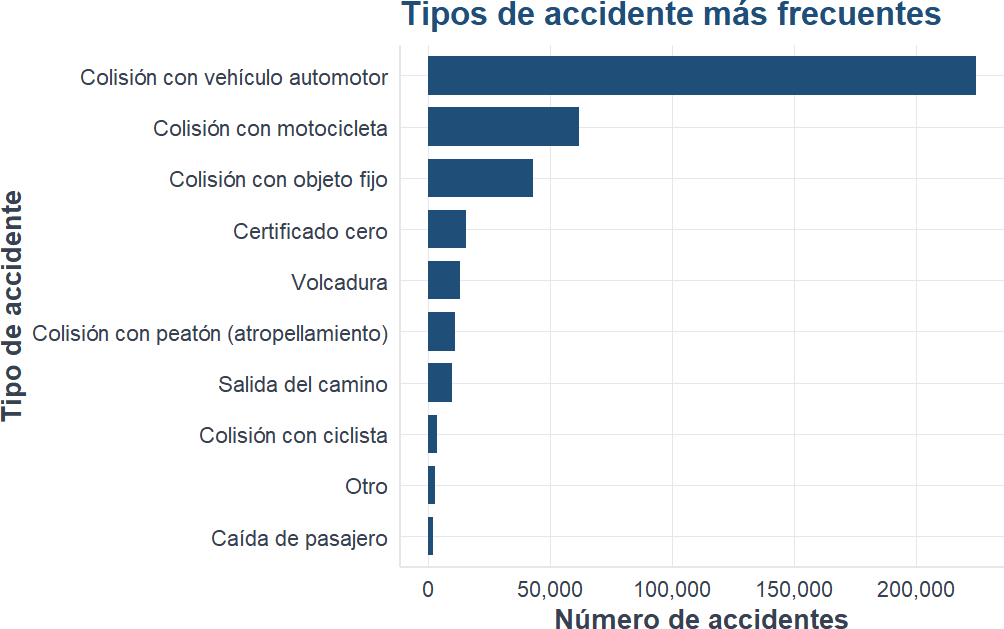
\includegraphics[keepaspectratio]{03-analisis-exploratorio_files/figure-pdf/unnamed-chunk-8-1.png}}

\section{Proporción por tipo de
accidente}\label{proporciuxf3n-por-tipo-de-accidente}

\pandocbounded{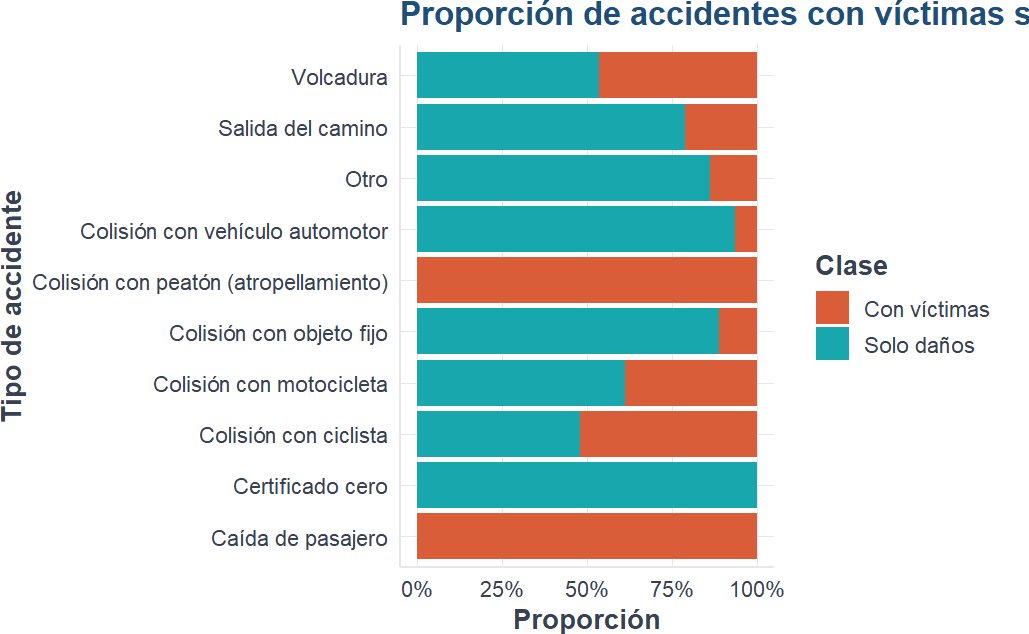
\includegraphics[keepaspectratio]{03-analisis-exploratorio_files/figure-pdf/unnamed-chunk-9-1.png}}

\section{Conclusión}\label{conclusiuxf3n-1}

El análisis exploratorio permite detectar patrones iniciales, revisar el
desbalance de clases e identificar variables útiles para modelar.

\bookmarksetup{startatroot}

\chapter{Regresión logística para
clasificación}\label{regresiuxf3n-loguxedstica-para-clasificaciuxf3n}

\section{Objetivos del capítulo}\label{objetivos-del-capuxedtulo-3}

Al finalizar este capítulo, el lector será capaz de ajustar una
regresión logística, predecir probabilidades y evaluar el desempeño.

\section{Fundamento matemático}\label{fundamento-matemuxe1tico}

La regresión logística utiliza la función:

\[
p=\frac{1}{1+e^{-z}}
\]

donde \(z=\beta_0+\beta_1x_1+\cdots+\beta_px_p\).

\section{Visualización de la función
logística}\label{visualizaciuxf3n-de-la-funciuxf3n-loguxedstica}

\pandocbounded{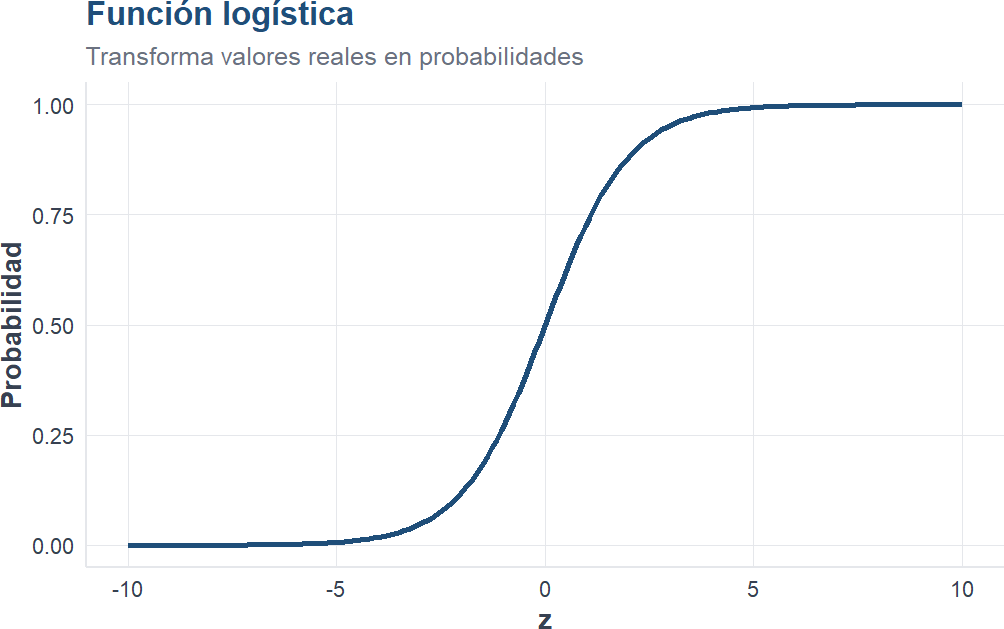
\includegraphics[keepaspectratio]{04-regresion-logistica_files/figure-pdf/unnamed-chunk-1-1.png}}

\section{Cargar paquetes y datos}\label{cargar-paquetes-y-datos}

\begin{verbatim}
[1] "Base preparada cargada correctamente."
\end{verbatim}

\section{Preparar y dividir datos}\label{preparar-y-dividir-datos}

\section{Ajustar modelo}\label{ajustar-modelo}

\begin{verbatim}
                Estimate   Std. Error     z value     Pr(>|z|)
(Intercept) 18.107257168 101.84719297  0.17778848 8.588891e-01
MES02       -0.045765700   0.02975556 -1.53805548 1.240350e-01
MES03       -0.032191364   0.02927313 -1.09968980 2.714673e-01
MES04       -0.002838049   0.02945462 -0.09635327 9.232400e-01
MES05       -0.015408552   0.02906672 -0.53010979 5.960358e-01
MES06       -0.054753129   0.02983667 -1.83509526 6.649158e-02
MES07       -0.076296781   0.03035194 -2.51373620 1.194598e-02
MES08       -0.094049541   0.02997105 -3.13801278 1.700975e-03
MES09       -0.077109438   0.03015044 -2.55748998 1.054306e-02
MES10       -0.154152374   0.02979697 -5.17342485 2.298416e-07
MES11       -0.106385033   0.02950811 -3.60528073 3.118157e-04
MES12       -0.111888509   0.02959338 -3.78086333 1.562855e-04
\end{verbatim}

\section{Predicción y matriz de
confusión}\label{predicciuxf3n-y-matriz-de-confusiuxf3n}

\begin{verbatim}
              Predicho
Real           Con víctimas Solo daños
  Con víctimas        13765       6739
  Solo daños          14302      82382
\end{verbatim}

\section{Métricas}\label{muxe9tricas}

\begin{verbatim}
  exactitud sensibilidad especificidad
1 0.8204509    0.6713324     0.8520748
\end{verbatim}

\section{Distribución de
probabilidades}\label{distribuciuxf3n-de-probabilidades}

\pandocbounded{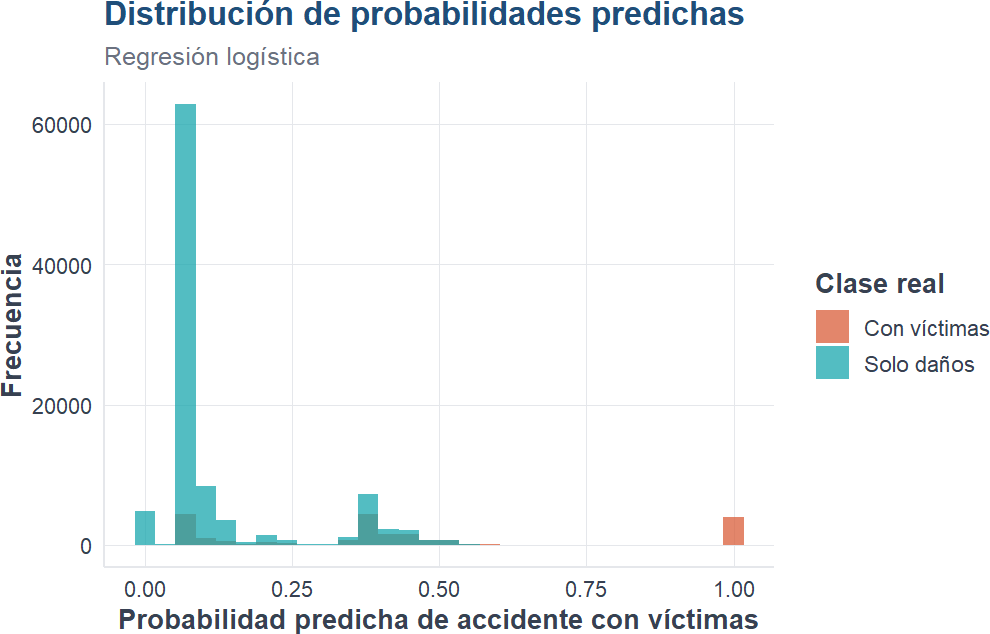
\includegraphics[keepaspectratio]{04-regresion-logistica_files/figure-pdf/unnamed-chunk-7-1.png}}

\section{Conclusión}\label{conclusiuxf3n-2}

La regresión logística es un modelo interpretable para clasificación
binaria. El punto de corte permite ajustar el balance entre sensibilidad
y especificidad.

\bookmarksetup{startatroot}

\chapter{k vecinos más cercanos,
k-NN}\label{k-vecinos-muxe1s-cercanos-k-nn}

\section{Objetivos del capítulo}\label{objetivos-del-capuxedtulo-4}

Al finalizar este capítulo, el lector será capaz de explicar k-NN,
preparar datos para este método, estandarizar variables y evaluar el
desempeño.

\section{Idea intuitiva}\label{idea-intuitiva}

k-NN clasifica una nueva observación según la clase más común entre sus
vecinos más cercanos.

\pandocbounded{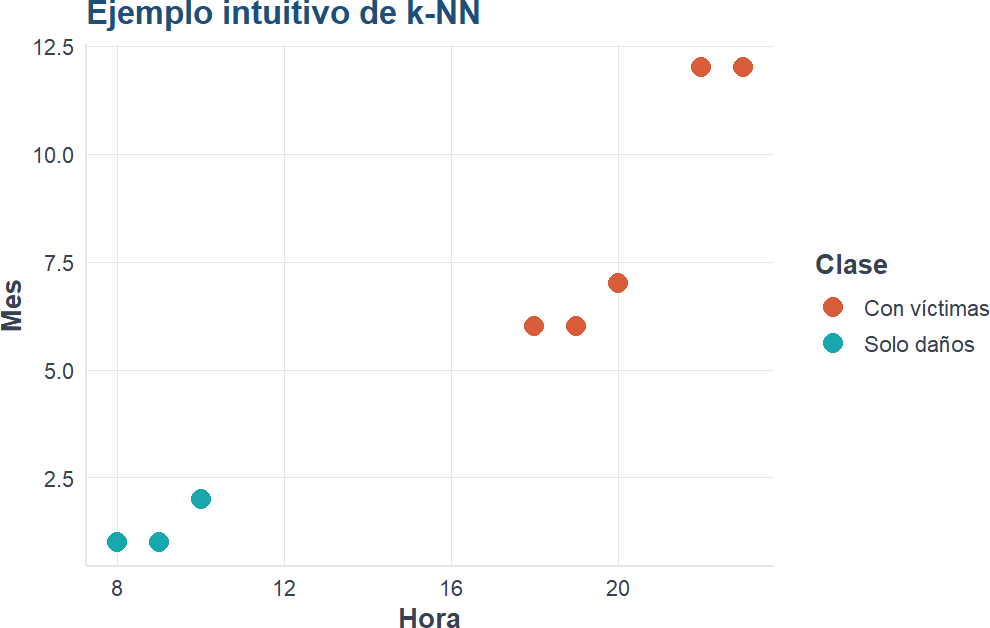
\includegraphics[keepaspectratio]{05-knn_files/figure-pdf/unnamed-chunk-1-1.png}}

\section{Distancia euclidiana}\label{distancia-euclidiana}

\[
d(A,B)=\sqrt{(x_1-x_2)^2+(y_1-y_2)^2}
\]

\begin{verbatim}
[1] 2.236068
\end{verbatim}

\section{Cargar y preparar datos}\label{cargar-y-preparar-datos}

\section{Modelo k-NN}\label{modelo-k-nn}

\begin{verbatim}
              Predicho
Real           Con víctimas Solo daños
  Con víctimas          211        399
  Solo daños            144       2846
\end{verbatim}

\section{Comparación de valores de
k}\label{comparaciuxf3n-de-valores-de-k}

\begin{verbatim}
   k exactitud sensibilidad especificidad
1  3 0.8433333    0.3770492     0.9384615
2  5 0.8480556    0.3491803     0.9498328
3 11 0.8558333    0.3377049     0.9615385
\end{verbatim}

\pandocbounded{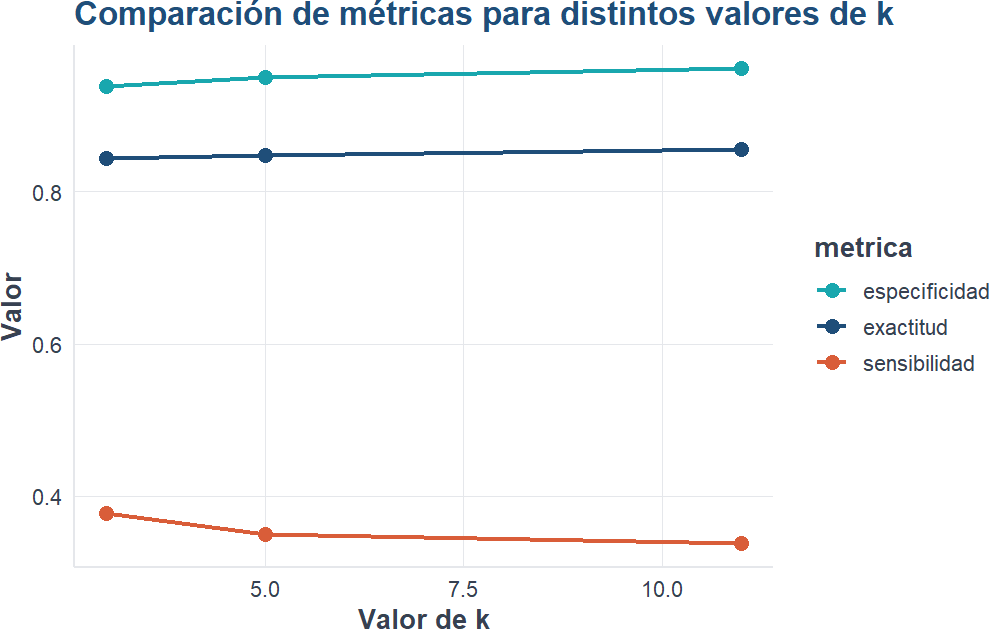
\includegraphics[keepaspectratio]{05-knn_files/figure-pdf/unnamed-chunk-6-1.png}}

\section{Conclusión}\label{conclusiuxf3n-3}

k-NN es un método intuitivo basado en similitud. Su desempeño depende
del valor de \(k\), del escalamiento y de la calidad de las variables
predictoras.

\bookmarksetup{startatroot}

\chapter{Árboles de decisión para
clasificación}\label{uxe1rboles-de-decisiuxf3n-para-clasificaciuxf3n}

\section{Objetivos del capítulo}\label{objetivos-del-capuxedtulo-5}

Al finalizar este capítulo, el lector será capaz de explicar la idea
básica de un árbol de decisión, entrenarlo en R y evaluar su desempeño.

\section{Introducción}\label{introducciuxf3n-2}

Los árboles de decisión clasifican observaciones mediante una secuencia
de preguntas. Son interpretables y pueden expresarse como reglas tipo
si-entonces.

\section{Fundamento matemático}\label{fundamento-matemuxe1tico-1}

Una medida común de impureza es el índice de Gini:

\[
Gini=1-\sum_{k=1}^{K}p_k^2
\]

\section{Cargar paquetes y datos}\label{cargar-paquetes-y-datos-1}

\begin{verbatim}
[1] "Base preparada cargada correctamente."
\end{verbatim}

\section{Usar la base completa}\label{usar-la-base-completa}

\begin{verbatim}
   filas columnas
1 390627        6
\end{verbatim}

\section{División y entrenamiento}\label{divisiuxf3n-y-entrenamiento}

\section{Complejidad e importancia}\label{complejidad-e-importancia}

\begin{verbatim}

Classification tree:
rpart(formula = accidente_con_victimas ~ MES + ID_HORA + DIASEMANA + 
    TIPACCID + CAUSAACCI, data = entrenamiento, method = "class", 
    control = rpart.control(cp = 0.005, minsplit = 1000, minbucket = 300, 
        maxdepth = 5))

Variables actually used in tree construction:
[1] TIPACCID

Root node error: 47604/273439 = 0.17409

n= 273439 

        CP nsplit rel error xerror      xstd
1 0.097051      0    1.0000 1.0000 0.0041653
2 0.005000      2    0.8059 0.8059 0.0038150
\end{verbatim}

\begin{verbatim}
   variable importancia
1  TIPACCID   22919.330
2 CAUSAACCI    1093.984
\end{verbatim}

\section{Gráfica opcional del
árbol}\label{gruxe1fica-opcional-del-uxe1rbol}

La gráfica completa del árbol puede ser pesada en PDF. El lector puede
ejecutarla manualmente en RStudio.

\section{Predicción y métricas}\label{predicciuxf3n-y-muxe9tricas}

\begin{verbatim}
              Predicho
Real           Con víctimas Solo daños
  Con víctimas         3965      16539
  Solo daños              0      96684
\end{verbatim}

\begin{verbatim}
  exactitud sensibilidad especificidad
1 0.8588678    0.1933769             1
\end{verbatim}

\section{Conclusión}\label{conclusiuxf3n-4}

Los árboles de decisión son modelos intuitivos, visuales e
interpretables. Este capítulo prepara el camino para modelos basados en
muchos árboles, como Random Forest.

\bookmarksetup{startatroot}

\chapter{Random Forest para
clasificación}\label{random-forest-para-clasificaciuxf3n}

\section{Objetivos del capítulo}\label{objetivos-del-capuxedtulo-6}

Al finalizar este capítulo, el lector será capaz de explicar Random
Forest, entrenar un modelo en R, interpretar importancia de variables y
evaluar desempeño.

\section{Introducción}\label{introducciuxf3n-3}

Random Forest combina muchos árboles de decisión. Cada árbol aprende
sobre una muestra aleatoria de los datos y la predicción final se
obtiene por votación mayoritaria.

\section{Fundamento matemático}\label{fundamento-matemuxe1tico-2}

Si se construyen \(B\) árboles, la predicción final es:

\[
\hat{y}(x)=\text{moda}\{\hat{y}^{(1)}(x),\hat{y}^{(2)}(x),\ldots,\hat{y}^{(B)}(x)\}
\]

\section{Cargar paquetes y datos}\label{cargar-paquetes-y-datos-2}

\begin{verbatim}
[1] "Base preparada cargada correctamente."
\end{verbatim}

\section{Muestra de trabajo}\label{muestra-de-trabajo}

\begin{verbatim}
  filas columnas
1 30000        6
\end{verbatim}

\pandocbounded{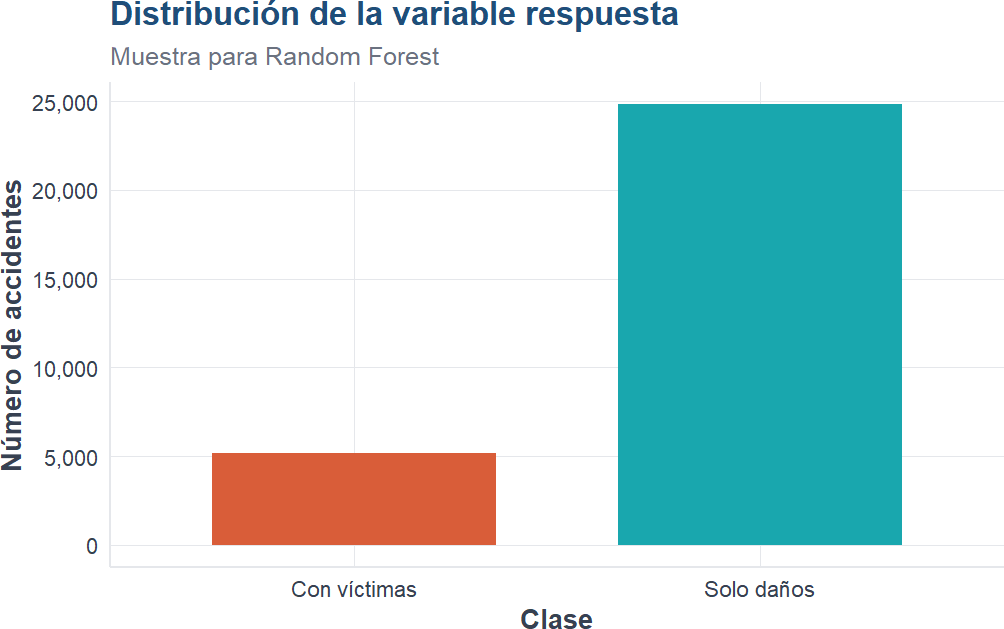
\includegraphics[keepaspectratio]{07-random-forest_files/figure-pdf/unnamed-chunk-3-1.png}}

\section{División en entrenamiento y
prueba}\label{divisiuxf3n-en-entrenamiento-y-prueba}

\begin{verbatim}
       conjunto registros
1 Entrenamiento     21000
2        Prueba      9000
\end{verbatim}

\section{Ajustar Random Forest}\label{ajustar-random-forest}

\begin{verbatim}
Ranger result

Call:
 ranger(accidente_con_victimas ~ MES + ID_HORA + DIASEMANA + TIPACCID +      CAUSAACCI, data = entrenamiento, num.trees = 200, mtry = 3,      min.node.size = 20, importance = "impurity", probability = TRUE,      seed = 123) 

Type:                             Probability estimation 
Number of trees:                  200 
Sample size:                      21000 
Number of independent variables:  5 
Mtry:                             3 
Target node size:                 20 
Variable importance mode:         impurity 
Splitrule:                        gini 
OOB prediction error (Brier s.):  0.1066668 
\end{verbatim}

\section{Importancia de variables}\label{importancia-de-variables}

\begin{verbatim}
   variable importancia
1  TIPACCID   1608.8347
2   ID_HORA    416.7870
3       MES    324.9780
4 DIASEMANA    234.4944
5 CAUSAACCI    220.5923
\end{verbatim}

\pandocbounded{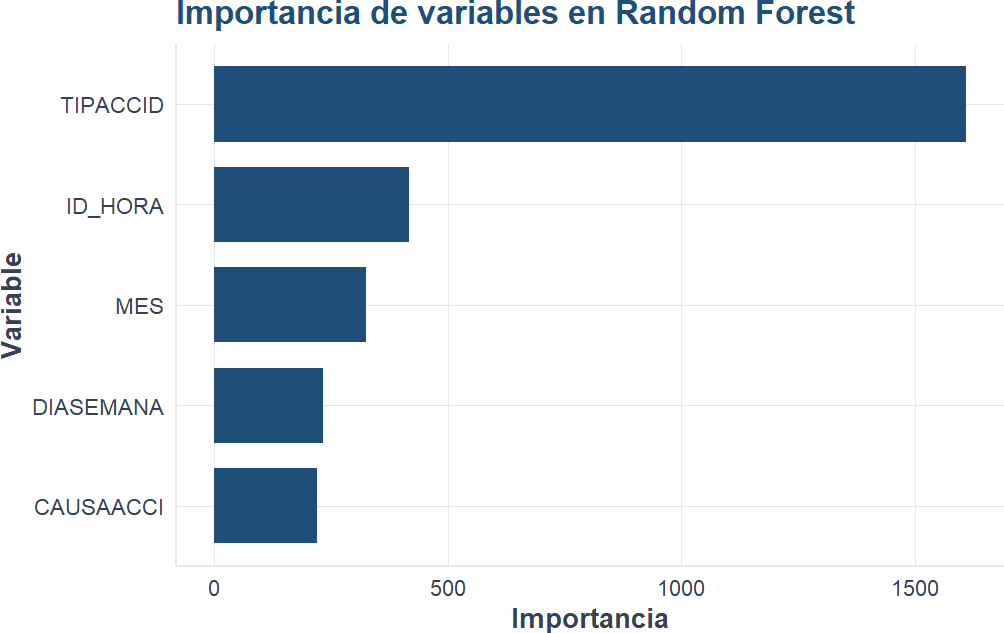
\includegraphics[keepaspectratio]{07-random-forest_files/figure-pdf/unnamed-chunk-7-1.png}}

\section{Predicción y métricas}\label{predicciuxf3n-y-muxe9tricas-1}

\begin{verbatim}
              Predicho
Real           Con víctimas Solo daños
  Con víctimas          475        991
  Solo daños            265       7269
\end{verbatim}

\begin{verbatim}
  exactitud sensibilidad especificidad
1 0.8604444    0.3240109     0.9648261
\end{verbatim}

\section{Distribución de probabilidades
predichas}\label{distribuciuxf3n-de-probabilidades-predichas}

\pandocbounded{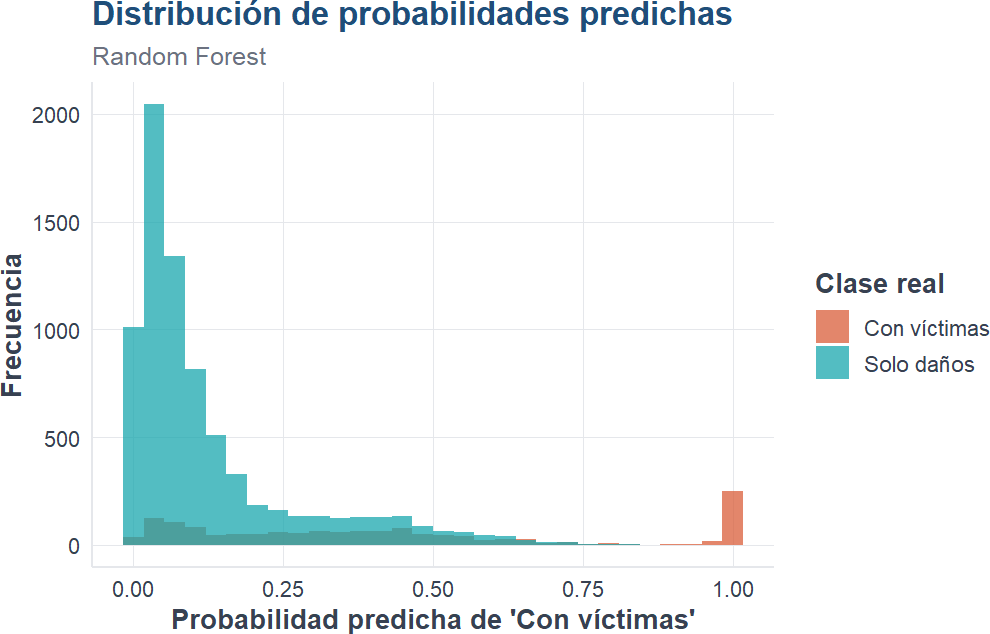
\includegraphics[keepaspectratio]{07-random-forest_files/figure-pdf/unnamed-chunk-10-1.png}}

\section{Conclusión}\label{conclusiuxf3n-5}

Random Forest mejora la estabilidad y la capacidad predictiva de un solo
árbol al combinar muchos árboles. Es uno de los métodos más útiles para
clasificación aplicada.


\backmatter


\end{document}
